\documentclass{../resources/acm_proc_article-sp}

\usepackage{todonotes}
\usepackage{fontspec}
\usepackage{makeidx}
\usepackage{rotating}

\usepackage{booktabs}
\usepackage{multirow}

\usepackage[
backend=biber,
style=numeric,
sorting=none
]{biblatex}
\addbibresource{../resources/lib.bib}
 
\setmonofont{DejaVu Sans Mono}
 
\pagenumbering{arabic}

\begin{document}

\title{Thesis Design}
\subtitle{Master Thesis Information Studies}

\author{
Jorick van Hees \\
\texttt{\textbf{Blue Billywig}}\titlenote{Blue Billywig, Catharina van Renneslaan 20, 1217 CX Hilversum, The Netherlands} \\
\texttt{jorick.vanhees@student.uva.nl} \\
\texttt{UvA Student Nr.: 10894020} \\
\texttt{VU Student Nr.: 2567527}
}

\maketitle

\category{Computing methodologies}{Computer vision}{Video summarisation}

\section{Introduction}

With the introduction of high speed internet and the introduction of video sharing platforms, the use of online video increased dramatically and is one of the main media content formats used on the web today, with increasing popularity in news media, business matters, education and the social web. According to \textcite{Cisco:2015wm}, 64 percent of the consumer internet traffic in 2014 was online video.

News media website navigation often exists of article pages and overview pages like the front page, designed to allow easy navigation to the article pages. The overview pages link to the article using a title, a small description and a visual preview. This visual preview, or thumbnail, is a small visual representation of the content. The thumbnail is only a few centimeters in size, depending on the implementation in the interface. The thumbnail should engage the user to follow the link to view the full article and is often the only visual reference.

Thumbnails have always been a strong visual cue for the user to find relevant content. A study from \textcite{Dziadosz:2002cl} in 2002 regarding thumbnails in their search engine results, showed that users made more accurate decisions when a thumbnail of the result was presented next to the textual result. In general, images tend to pull the audience to the content; it's what newspapers are doing for years with the big frontpage images. The contents of these thumbnails exist of stock photos, actual photos from the event, or other designed images containing company logos, previews of graphs and other relevant visuals. Overview pages linking to multiple news articles often use these thumbnails to improve the visual appearance of the website, but also try to invite the user into viewing the article. These images have always been static, but with the increase of broadband internet speeds and reliability (even on mobile devices), opportunities arise to create moving thumbnails. These thumbnails may improve the user experience and could increase the chances of users watching the full article.

\begin{figure}[h]
  
\includegraphics[width=\linewidth]{images/belfast-telegraph-thumbnail}
  \caption{Screencapture of the Belfast Telegraph frontpage (http://www.belfasttelegraph.co.uk/) on the 5th of february, showing a thumbnail.}
\end{figure}


\section{The moving thumbnail}

In a lot of ways, the moving thumbnail is the same as a regular static thumbnail with the exception that it contains `moving images'. It is located in the same positions on websites and behaves the same way when the user interacts with it (a click on the thumbnail directs the user to the article). Depending on the medium of the full content (an article, video or image), the thumbnail is often a summarised substitution.

Static thumbnails have different purposes in news media websites in relationship to the content: it can try to accurately describe the content, or it can attempt to invite the user to view the full content (which is what we can call a teaser). The chosen role of the thumbnail depends heavily on the type of content, the strategic goals of the media company and the location of where the thumbnail is used. Since the moving thumbnail replaces the static thumbnail, it should serve the same purpose.

To pick the best (static) thumbnail for a desired goal, a number of systems exist to aid an editor into selecting a thumbnail. The most simple system features a time selector and a preview window in which the editor is able to select a frame on a certain time to use as thumbnail. Other systems use different video analysis techniques to propose a set of suitable options to the editor. In order to use a moving thumbnail as a replacement for the static thumbnail, the creation of these moving thumbnails should be fast and convenient.

\subsection{New challenges for moving thumbnails}

Thumbnails are not the main focus of the page, and will not be started by a user action like a regular video would by clicking a play button. The users attention might also not directly be focussed on the moving thumbnail, and sometimes even multiple moving thumbnails may show on a page. These issues are also present in static thumbnails, but since they have no dimension of time, this does not present itself as an issue. The workings and design of a moving thumbnail should account for this lack of initial focus.

A static thumbnail will show only a single frame of the original video, revealing little of the actual content. A moving thumbnail however, might already show the punch line of the video, eliminating the need for a user to click through to the full video. For end-users, this might not impose as a problem, however media companies gain their revenues by serving advertisements before a video, or next to an article. This highlights the need to create moving thumbnails that tease the user, instead of showing a summary.

A more technical challenge is the design of the moving thumbnail in relation to processing power, internet speeds and device limitations. Even small videos can be significantly larger in file size than static thumbnails, and may consume more processing power, especially on mobile devices. The technical details of the moving thumbnail should consider these limitations.

\section{Problem statement}
\label{sec:problem statement}

Creating moving thumbnails manually for every video can be a time consuming task, even when presented with various editing tools that allow quick trimming. In order to solve this problem,  automatic generation of moving thumbnails is essential for the use and implementation of this new concept.

To the best of our knowledge, there is no system that generates moving thumbnails with the goal to invite the user to view the full video. The specifications and requirements for a moving thumbnail are unclear, a method to measure the effectiveness of the output of the system does not exist for this particular case, and since the concept is new, there is no data available to accurately train a system for this purpose.

The absence of data leads the core of this research: The goal is to build a system that generates moving thumbnails and evaluates the results automatically to validate the output and allows for rapid improvements without user testing. The automatic evaluation can not rely on real world data (since it does not exist yet) and functions as some sort of sanity check. When the system scores acceptable on the automatic evaluation, the results are implemented in an end user test scenario to evaluate the system and gain real world data for the purpose of generating moving thumbnails.

The research question is as follows:

\textbf{How can we build a system that automatically generates moving thumbnails that invite the user to view the full video?}

The system that automatically generates moving thumbnails from a video has to take several factors into account. These factors range from specifications like size, length and audio, to more content focussed factors: Does the moving thumbnail accurately reflect the full video and does it invite users to actually do so? These factors form an important subject in the design of the system. They will be based on existing previous research in the field of static thumbnail generation, video navigation and video summarisation. These factors lead to the first subquestion:

\textit{What features play a role in the automatic generation of moving thumbnails?}

There is no data at hand that allows us to benchmark to our moving thumbnails. This means that there is no way of telling that changes made to our system improve the result. In order to solve this issue, we need to include an automatic evaluation that gives us a guideline when improving the system. The need for an automatic evaluation is a result of the available resources for real world user testing. This leads us to the second subquestion:

\textit{How can the automatic thumbnail generator be automatically evaluated?}

Since the automatic evaluation only offers a guideline and will have no definitive answer to our main question, a real world user study will be done to conclude the research. The result of this study can confirm and validate the results of the automatic evaluation, and will benchmark the generated moving thumbnails with actual users. This concludes into our final subquestion:

\textit{How does the output of the system behave in a real world scenario?}

By answering these questions, we can describe a system that automatically generates moving thumbnails and evaluates its results, which are validated by a real world survey.

\subsection{Context}

The origin of the new concept of moving thumbnails lies at media companies, who constantly try to seek new ways to improve their website and the way users navigate their news. At Blue Billywig, we received a request to offer a way to show moving thumbnails, created manually by the editors. After investigating this new opportunity, it was decided that an automatic way of generating these moving thumbnails was required.

Blue Billywig is a company that builds and maintains a video management systems, in which its customers can upload videos, edit metadata, adjust the way these videos are displayed and publish the videos on their website. In a lot of ways, the systems works the same way as the populair video site YouTube does \cite{YouTube:A-l2msAp}, only focussed on the use by companies and without a community.

\section{Approach}

As mentioned in section \ref{sec:problem statement}, the research can be divided into three closely related subjects. The first subject is the moving thumbnail generator itself, a system that uses various features to determine what to use from an input video to create a moving thumbnail as output. The second subject is a validator that automatically validates the output of the system, to check the integrity of the generated moving thumbnails. The third subject is the user test scenario that tests the output of the generator with actual users, which results can in turn be used to compare the validator results with the actual user testing, and show real world effectiveness of the thumbnail generator. This workflow is shown in figure \ref{fig:workflow}. These three subjects combined form a study that covers all grounds in this new concept of automatically generating thumbnails.

\begin{figure}[h]
  \label{fig:workflow}
  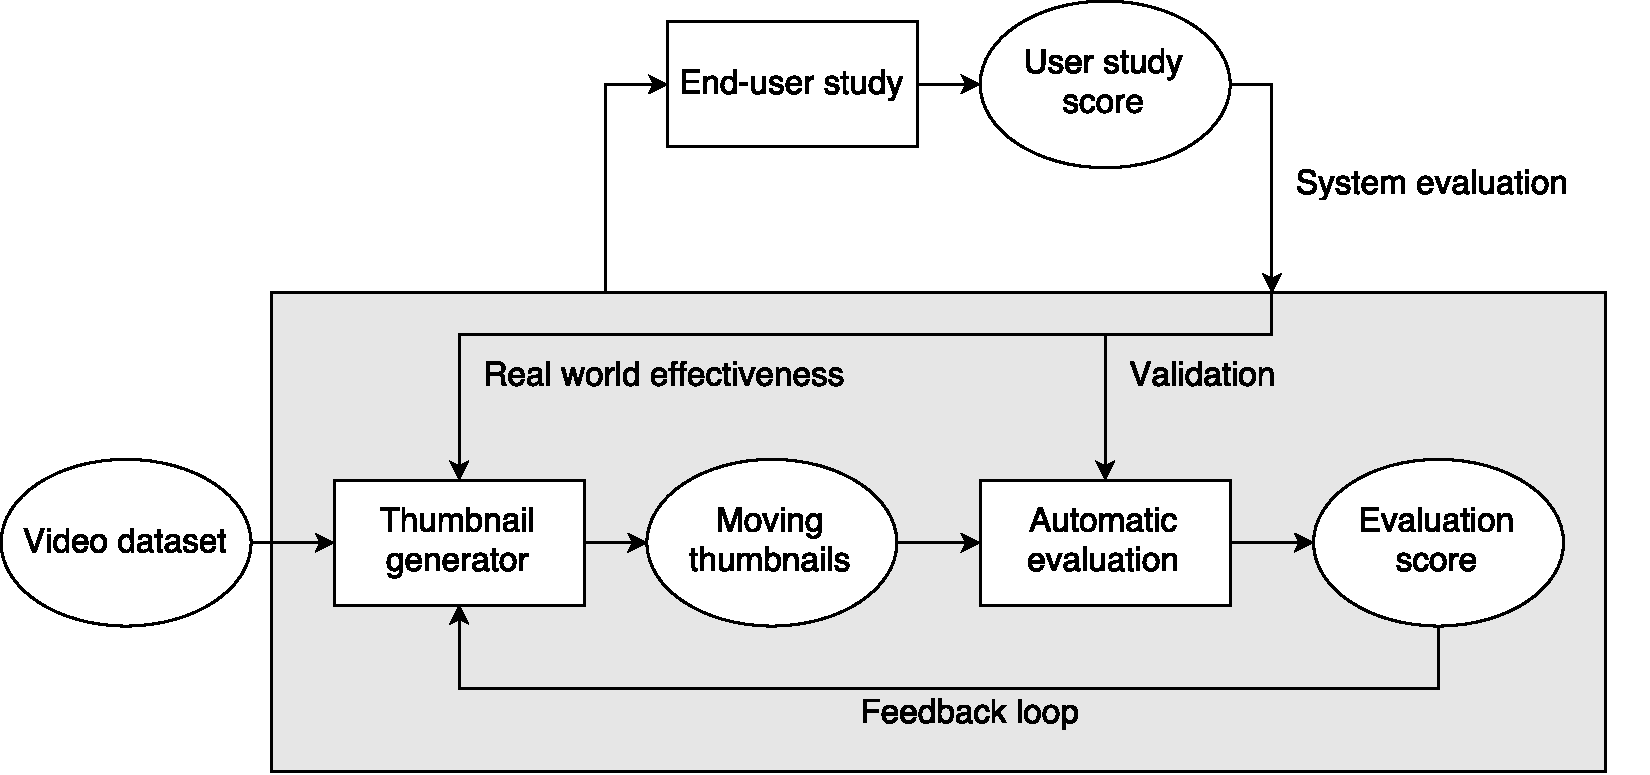
\includegraphics[width=\linewidth]{images/thesis-system.pdf}
  \caption{Schematic workflow overview of the complete system, showing feedback directions on the generator and evaluation.}
\end{figure}

\subsection{The dataset}

The dataset that will be used has a number of specific requirements. In our scenario, the moving thumbnail will be primarily used on article overview pages on news websites. This means that the dataset will include only videos from that domain, most preferably from a single selected news agency. Since there are multiple ways to generate video summaries, using internal and external data from the video, the dataset should provide in both ways. This means that the internal data (meaning the video itself) should be easily be accessible, and that external data (meaning metadata like title, tag and description) should be present. The required size of the dataset should be around the hundreds of videos, based on earlier research in video summarisation \cite{Almeida:2012be,Christel:2004in,Money:2008fn}.

\section{Literature study}

The generation of moving thumbnails is a new concept, relating close to a number of other domains: Video navigation and interfaces, static thumbnail generation and video summarisation.

\subsection{Video navigation}

There are a lot of interfaces designed to assist humans in navigating a video library. A summary by \textcite{Schoeffmann:2010iw} describes over 40 different interfaces that use different techniques to allow convenient browsing through a collection of videos. These range from displaying a key frame best describing the video, or a collection of keyframes with their sizes related to the importance of the frame. Most of these interfaces have some sort of system that automatically determines what to display on the screen, taken into consideration the different conditions in which the system is used. A study by \textcite{Hurst:2011jx} describes a user study to the recognition of video using different thumbnail sizes, numbers and various movement in the thumbnails. The study shows that users are able to handle multiple small thumbnails on mobile devices, especially when the thumbnails included motion. Since one of the goals of the moving thumbnail is to improve the navigation of users in a news media website, video navigation literature could especially prove useful in the design and implementation of moving thumbnails in overview pages.

\subsection{Static thumbnail generation}

The issue of video navigation using thumbnails has been an active topic of research. A \citeyear{Kim:2015co} study by \textcite{Kim:2015co} describes a system that automatically combines video frames to generate a thumbnail containing more information that a single frame. Another study describes thumbnail candidate selection using image quality evaluation \cite{Zhang:2014jg}. A combination of internal and external analysis of the video content to select thumbnails is used by a study by \textcite{Liu:2015ux}. The techniques and analysation methods used in these systems can possibly be of use when evaluating the generated moving thumbnails.

Many systems that generate thumbnails use a ranking of different frames to propose a suitable thumbnail \cite{Choi:2015gm,Zhang:2012eo,Gao:2009dx}. In static thumbnail generation, this ranking can be used to select the best thumbnail. In moving thumbnail generation (or other video navigation interfaces) the ranking can be used to create a composition of the video. This creates opportunities to generate moving thumbnails that consist of different shots from the original video.

\subsection{Video summarisation}

Video summarisation is the domain that is closest to the concept of the moving thumbnail, since a moving thumbnail is basically a video summarisation with a few major differences. The length of a video summary would depend on the contents of the actual video, an hour long video would need a longer summary to contain all concepts in the video than a summary for a minute long video. The moving thumbnail however, should ideally always be around the same size, since it only has to attract users to view the full video, instead of showing what the video is about.

Techniques for video summarisation can be divided into three different categories: Internal analysis, external analysis and a hybrid of the two. Internal analysis techniques use information that is gained from analysing the video itself, while external analysis uses the information available outside the video (metadata like title, description or tags). The hybrid techniques combine both internal and external analysis \cite{Money:2008fn}.

The knowledge gained from video summarisation can be used to generate and extract relevant parts from a video, and those in turn can be used to create moving thumbnails. The difference between video summarisations and moving thumbnails has to be highlighted in order to modify (or use techniques from) video summarisation techniques in order to use them for another purpose. Various frameworks and surveys on different techniques highlight the differences and effectiveness in domains and content \cite{Money:2008fn,Ajmal:2012hi}, which might be useful in the design of the moving thumbnail generator.

\section{Planning}

Development of the system will be planned in a scrum-like planning, implemented in the scrum planning of Blue Billywig. This means that the planning is divided into sprints of two weeks. The planning, as shown in table \ref{table:planning} on page \pageref{table:planning}, describes a number of topics that should be covered in those sprints. The column `BB' describes the sprint numbers as used in the Blue Billywig sprint planning.

Working on the master thesis document itself is done throughout the whole planning, and has no defined deadlines other than the draft versions in sprint 9 and 10. It should be noted that most subjects are addressed in each sprint, with a main focus on certain subjects as described in the `Main focus' column.

\subsection{Plan B}

One of the highest priorities in the system is the user study. Without the user study, the results of the system, as well as the effectiveness of the validator cannot be measured. Thus, it is important that the user study is ready in sprint 6 to gather enough data to gain significance. Sprint 5 is mostly used to improve the overal system, and can be changed when the workflow isn't properly set up in sprint 4. The overall planning can be extended with one sprint by removing one of the draft versions of the master thesis. However, this should be an extreme measure when the system has severe delays and the system can not be validated yet.

\printbibliography

\balancecolumns

\begin{table*}[]
\centering
\caption{Planning}
\label{table:planning}
\resizebox{\textwidth}{!}{%
\begin{tabular}{llcll}
\hline
\textbf{Date}                 & \textbf{Week} & \textbf{Sprint}              & \textbf{BB}                    & \textbf{Main focus}                                                                               \\ \hline
Friday, February 12, 2016     & 7             & \multirow{2}{*}{\textbf{1}}  & \multirow{2}{*}{5.46}          & \multirow{2}{*}{Thesis design setup, dataset acquisition, useable feature search in literature}   \\
Friday, February 19, 2016     & 8             &                              &                                &                                                                                                   \\
Friday, February 26, 2016     & 9             & \multirow{2}{*}{\textbf{2}}  & \multirow{2}{*}{5.47}          & \multirow{2}{*}{Dataset acquisition \& analysis, feature extraction library, workflow setup}      \\
Friday, March 4, 2016         & 10            &                              &                                &                                                                                                   \\
Friday, March 11, 2016        & 11            & \multirow{2}{*}{\textbf{3}}  & \multirow{2}{*}{5.48}          & \multirow{2}{*}{Dataset preperation, feature libraries in workflow, dataset analysis in workflow} \\
Friday, March 18, 2016        & 12            &                              &                                &                                                                                                   \\
Friday, March 25, 2016        & 13            & \multirow{2}{*}{\textbf{4}}  & \multirow{2}{*}{5.49}          & \multirow{2}{*}{Literature on features, first full workflow \& results}                           \\
Friday, April 1, 2016         & 14            &                              &                                &                                                                                                   \\
Friday, April 8, 2016         & 15            & \multirow{2}{*}{\textbf{5}}  & \multirow{2}{*}{5.50}          & \multirow{2}{*}{Improvements in overal system design, feedback loop implementation.}              \\
Friday, April 15, 2016        & 16            &                              &                                &                                                                                                   \\
Friday, April 22, 2016        & 17            & \multirow{2}{*}{\textbf{6}}  & \multirow{2}{*}{5.51}          & \multirow{2}{*}{User study test design, system output preparation.}                               \\
Friday, April 29, 2016        & 18            &                              &                                &                                                                                                   \\
Friday, May 6, 2016           & 19            & \multirow{2}{*}{\textbf{7}}  & \multirow{2}{*}{5.52}          & \multirow{2}{*}{User study}                                                                       \\
Friday, May 13, 2016          & 20            &                              &                                &                                                                                                   \\
\textbf{Friday, May 20, 2016} & \textbf{21}   & \multirow{2}{*}{\textbf{8}}  & \multirow{2}{*}{\textbf{5.53}} & \multirow{2}{*}{\textbf{Mid-term presentation, second reader + defence date}}                     \\
Friday, May 27, 2016          & 22            &                              &                                &                                                                                                   \\
Friday, June 3, 2016          & 23            & \multirow{2}{*}{\textbf{9}}  & \multirow{2}{*}{5.54}          & \multirow{2}{*}{Thesis draft version 1, User study evaluation}                                    \\
Friday, June 10, 2016         & 24            &                              &                                &                                                                                                   \\
Friday, June 17, 2016         & 25            & \multirow{2}{*}{\textbf{10}} & \multirow{2}{*}{5.55}          & \multirow{2}{*}{Thesis draft version 2, discussion, final touches, presentation.}                 \\
Friday, June 24, 2016         & 26            &                              &                                &                                                                                                   \\
\textbf{Friday, July 1, 2016} & \textbf{27}   & \textbf{11}                  & \textbf{5.56}                  & \textbf{Master Thesis Deadline}                                                                   \\
Friday, July 8, 2016          & 28            & \textbf{}                    &                                & \textit{Defence}                                                                                  \\
Friday, July 15, 2016         & 29            & \textbf{}                    &                                & \textit{Defence}                                                                                  \\
Friday, July 22, 2016         & 30            & \textbf{}                    &                                & \textit{Defence}                                                                                  \\
Friday, July 29, 2016         & 31            & \textbf{}                    &                                & \textit{Defence}                                                                                  \\ \hline
\end{tabular}
}
\end{table*}

\end{document}
